\section{Framtagande av arkitektur}
Det här kapitlet tar upp de arkitektoniska mekanismer som behövs för att ta fram en arkitektur för applikationen.
\subsection{Systemanatomi}
Systemanatomin har tagits fram baserat på de funktionella kraven från kravspecifikationen och användningsfall.
\begin{figure}[h]
    \centering
    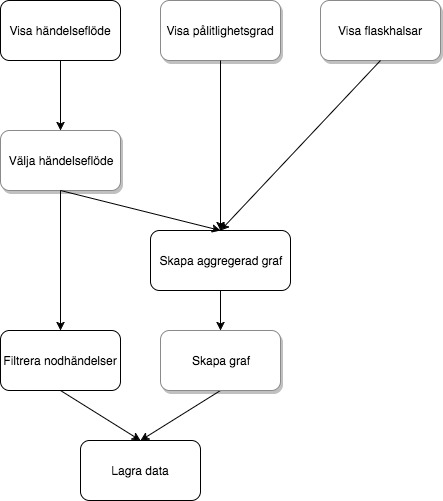
\includegraphics[scale=0.5]{Systemanatomi}
    \caption{Systemets anatomi.}
    \label{fig:systemanatomi}
\end{figure}
\ \\
I figur \ref{fig:systemanatomi} visas systemanatomin för applikationen. Systemanatomins primära användarfunktioner är högst upp i figuren.
\subsection{Framtagande av prototyp}
Tillsammans med krav från kravspecifikationen och kundmöten så utformades en prototyp av användargränssnittet. Den konkretiserar den funktionalitet som produkten behöver och klargör användargränssnittets grafiska representation. Fördelar med att göra en prototyp av den tänkta färdiga applikationen är att återkoppling fås från kunden under ett tidigt stadie och därmed kan arkitekturen anpassas bättre efter kundens krav. En prototyp togs fram och presenterades till kund, efter återkoppling kunde en ny version tas fram. 
\newpage
\subsubsection{Prototyp}
I den här delen presenteras den prototyp som togs fram efter återkoppling av kund. Den visar de tre olika nivåerna applikationen har. Dessa är aggregeringsvyn med de aggregerade graferna, tabelläge med de underliggande händelserna från en nod i aggregeringsvyn och händelseflöde som är en specifik händelse från tabelläge.
\begin{figure}[h]
    \centering
    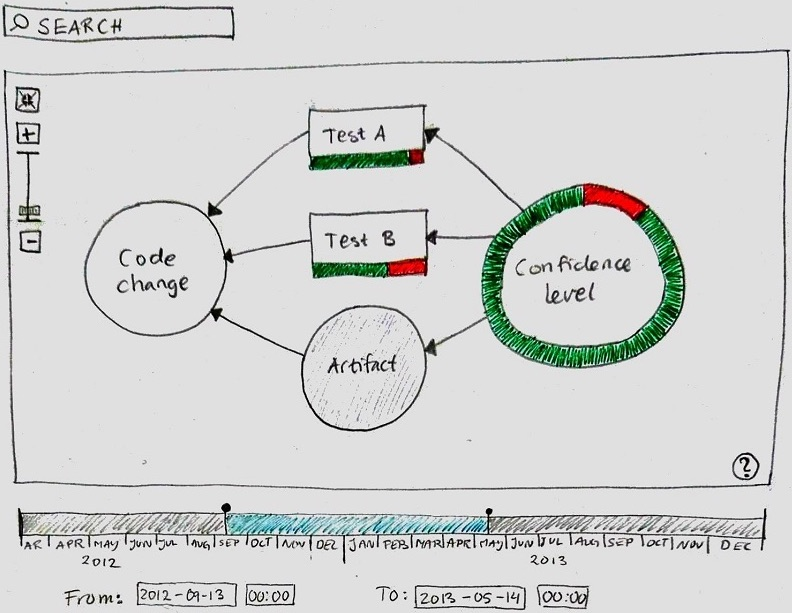
\includegraphics[scale=0.2]{niva1}
    \caption{Prototypens aggregeringsvy: nivå 1.}
    \label{fig:architectuarl_prototype1}
\end{figure}
\ \\
\begin{figure}[h]
    \centering
    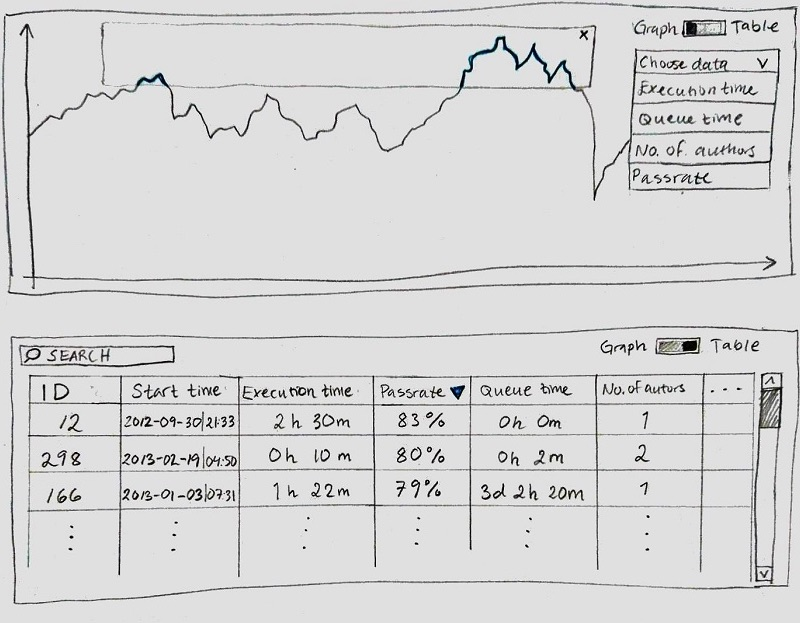
\includegraphics[scale=0.2]{niva2}
    \caption{Prototypens tabelläge: nivå 2.}
    \label{fig:architectuarl_prototype2}
\end{figure}
\ \\
\begin{figure}[h]
    \centering
    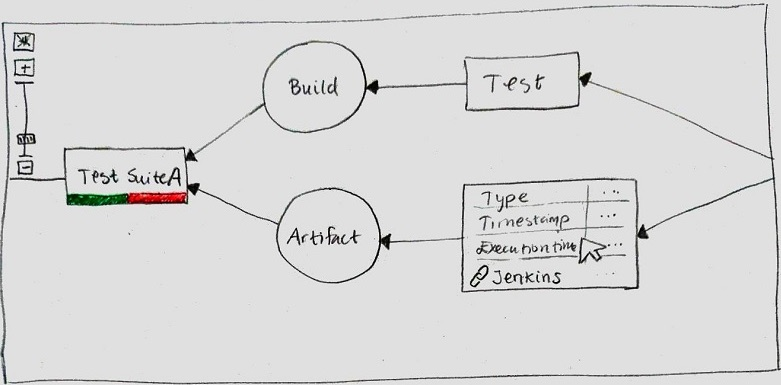
\includegraphics[scale=0.3]{niva3}
    \caption{Händelseflöde: nivå 3.}
    \label{fig:architectuarl_prototype3}
\end{figure}
\ \\
\newpage
\subsection{Val av arkitektur}
En systemskiss togs fram för att ge en översiktlig beskrivning av den applikation som skulle tas fram.
\begin{figure}[h]
    \centering
    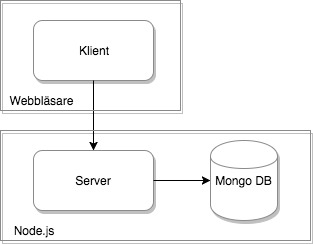
\includegraphics[scale=0.6]{Systemskiss}
    \caption{Den framtagna systemskissen av applikationen.}
    \label{fig:architectural_overview}
\end{figure}
\ \\
Baserat på den prototyp som gjordes kunde en systemskiss tas fram för applikationen som kan ses i figur \ref{fig:architectural_overview}. Det ska finnas en del som visualiserar datan och en databas där Eiffeldatan lagras. För att kunna välja ut den data som ska visualiseras hos klienten behövs en server. Meteor består av en klient och en server, där servern har en integrerad databas. Av abstraktionskäl så valdes att se servern och databasen som två separata lager. Applikationen använder sig av Meteors standard för strukturering av filer vilket ger en tydlig separation av klient och server.\cite{website:meteorstructure} Applikationen får därmed en trelagerarkitektur där den har ett presentationslager som sköter allt relaterat till visualisering, en server som sköter all hanteringen av data och en databas att förvara Eiffelhändelserna.
\newpage
\section{Trelagerarkitektur}
Den trelagerarkitektur som hade valts presenteras i denna del av kapitlet och även den funktionalitet som varje lager har.
\begin{figure}[h]
    \centering
    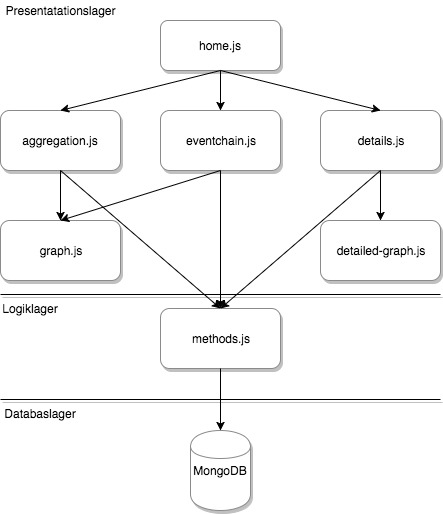
\includegraphics[scale=0.5]{Trelagerarkitektur}
    \caption{Den framtagna arkitekturen för applikationen.}
    \label{fig:layer_architecture}
\end{figure}
\ \\
Den lagrade arkitekturen som togs fram är separerat i tre olika lager som kan ses i \ref{fig:layer_architecture}. De tre lagren som applikationen består av är presentationslager, logiklager och databaslager.
\subsection{Presentationslager}
Presentationslagret är där all funktionalitet för visualisering finns. Det är Meteorklienten som är detta lager. Det finns tre filer: aggregation.js, details.js och eventchain.js som är de filer som innehåller all funktionalitet för de olika nivåerna i applikationen. \\
\begin{itemize}
  \item \texttt{aggregation.js} - innehåller de funktionsanrop som de aggregerade graferna behöver i aggregeringsvyn.
  \item \texttt{eventchain.js} - innerhåller de funktionsanrop som behövs när det är en nod från den aggregerade grafen som ska visas i tabelläget.
  \item \texttt{details.js} - innerhåller de funktionsanrop för händelseflödet och ska precis som \texttt{aggregation.js} rendera grafer.
  \item \texttt{graph.js} - är där all rendering av grafer sker. \texttt{graph.js} använder sig av två externa JavaScript bibliotek: Cytoscape.js för rendering av graferna och Dagre.js för dess layout.\cite{website:cytoscape}\cite{website:dagre}
  \item \texttt{detailed-graph.js} - är där all funktionalitet för tabelläget finns. Den använder sig av ett externt JavaScript bibliotek Vis.js.\cite{website:vis}
\end{itemize}
\newpage
\subsection{Logiklager}
Logiklagret är applikationens Meteorserver där det är methods.js som sköter hämtningen av data från databaslagret.
\subsection{Databaslager}
Applikationens databas är av typen MongoDB och det är där de Eiffelhändelser förvaras.\cite{website:mongodb} Den är integrerad i Meteorservern men är separerad av abstraktionsskäl för att tydliggöra gränsen mellan server och databas. 